\documentclass{article}
\usepackage[utf8]{inputenc}
\usepackage[spanish]{babel}
\usepackage{listings}
\usepackage{graphicx}
\graphicspath{ {images/} }
\usepackage{cite}




\begin{document}

\begin{titlepage}
    \begin{center}
        \vspace*{1cm}
            
        \Huge
        \textbf{Informe de Análisis y Diseño Parcial 1}
            
        \vspace{0.5cm}
        \LARGE
        %Subtítulo
            
        \vspace{1.5cm}
            
        \textbf{YESIKA MILENA CARVAJAL DÍAZ}
        \textbf{NICOLL CAROLINE CHAZATAR}\\
        \textbf{ANDRES FELIPE ZULUAGA ORTÍZ}
            
        \vfill
            
        \vspace{0.8cm}
            
        \Large
        Departamento de Ingeniería Electrónica y Telecomunicaciones\\
        Universidad de Antioquia\\
        Medellín\\
        21 de Febrero de 2022
            
    \end{center}
\end{titlepage}

\tableofcontents
\newpage

\section{INTRODUCCIÓN}

\section{RESÚMEN}

\section{OBJETIVOS}

\subsection{GENERALES}

\subsection{ESPECÍFICOS}

\section{METODOLOGÍA}

El proyecto se divide en 6 bloques:

\begin{enumerate}
\item PC1: Recibe los datos vía serial y es el encargado de enviar los datos al primer Arduino.

\item Sistema de generación de información serial:  Este es el primer Arduino, el cual recibe la información que envía el PC1, y envía señal de datos y reloj. Los cuáles reciben el segundo Arduino, y el sistema de paralelización.

\item Sistema que paraleliza los datos:  En este bloque, se paraleliza la información de un byte, es decir, esta recoge un byte y lo separa en 8 bits independientes. Los 8 bits independientes entran paralelamente al circuito de verificación de la banda (sistema de desencriptación). La paralelización de los datos se realiza por medio del circuito integrado 74HC595.

\item Sistema de desencriptación: Este sistema recibe los datos binarios paralelizados y con respecto a estos se genera de salida una bandera. Si la bandera es verdadera, significa que el próximo byte será el mensaje real. Este sistema se crea con base al byte que verifica el ingreso del mensaje real, y se realiza con compuertas lógicas.

\item Sistema de recepción: Este sistema tiene tres entradas: los datos, la señal del reloj y la bandera de verificación del mensaje real. Los datos y la señal del reloj se ingresan desde el sistema de generación de información serial, y la bandera entra desde el sistema de desencriptación. El sistema de recepción almacena el dato correspondiente al mensaje real para posteriormente entregarlo al Arduino 2. La señal del reloj sirve para indicarle al sistema de recepción en qué momento empieza la recolección del mensaje real, la cual es de 8 flancos de subida o de bajada del reloj después de la activación de la bandera. Este bloque se encuentra en el Arduino 2.
PC2: Este bloque recibe la señal del mensaje real, desde el sistema de recepción, y lo reproduce en una pantalla LCD.

\end{enumerate}

\subsection{Circuito integrado 74HC595}\\
El circuito integrado es útil en la realización de la práctica en la creación del bloque Sistema que paraleliza los datos. El 74HC595 nos ayuda a paralelizar los bytes en sus 8 puertos de salida para que estos entren al Sistema de desencriptación.\\

Los pines de alimentación del integrado son el pin 8 para tierra y 16 para Vcc.\\

Se debe generar una diferencia de potencial en los pines MA y OE para habilitar las salida del integrado, por lo que el pin OE se conecta a tierra y MA a Vcc.\\

Los pines SH-CP(11), DS(14), ST-CP(12) controlan el ingreso de los bits que se reproducen en las salidas del integrado. El pin DS da el valor del bit, el SH-CP es la señal para tomar el bit de DS, y ST-CP muestra los bits almacenados previamente en las salidas del integrado. Las señales reproducidas inician desde la salida Q0 hasta Q7, que corresponden respectivamente a los pines 15 y 1-7.\\


\begin{figure}[h]
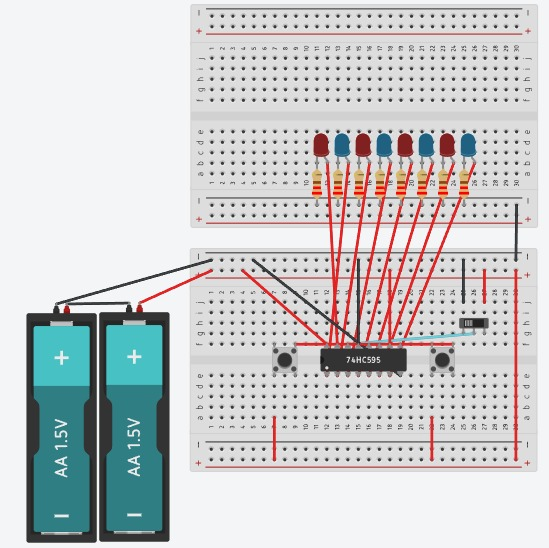
\includegraphics[width=7cm]{74HC595.jpg}
\centering
\caption{Circuito independiente 74HC595.}
\label{fig:74HC595.jpg}
\end{figure}




\subsection{Comunicación entre Arduinos}\\




\section{DESARROLLO}



\section{CONCLUSIONES} \label{conclulsion}

    

\bibliographystyle{IEEEtran}
%\bibliography{references}

%\cite{referencia}

\end{document}
